% ----------------------------------------------------------
% FIGURE: CWSL response surface vs cost ratio R
% ----------------------------------------------------------
\begin{figure}[t]
\centering
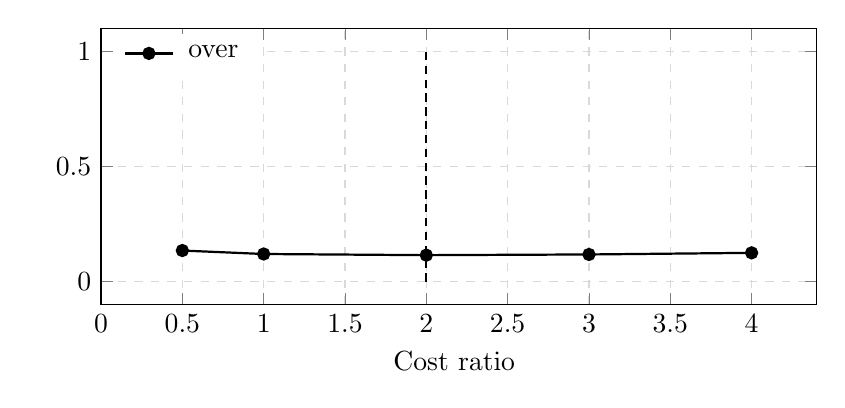
\begin{tikzpicture}
\begin{axis}[
    width=0.88\textwidth,
    height=0.42\textwidth,
    xlabel={Cost ratio $\R{}$},
    ylabel={$\CWSLR{}$},
    xmin=0,
    ymajorgrids=true,
    xmajorgrids=true,
    grid style={dashed,gray!30},
    legend style={draw=none, at={(0.02,0.98)}, anchor=north west},
    legend cell align={left},
]

% --- Placeholder curve (replace with your computed values) ---
% Example grid: R in {0.5, 1.0, 2.0, 3.0, 4.0}
\addplot[
    thick,
    mark=*,
]
coordinates {
    (0.5, 0.135)
    (1.0, 0.120)
    (2.0, 0.115)
    (3.0, 0.118)
    (4.0, 0.125)
};
\addlegendentry{$\CWSLR{}$ over $\Rgrid{}$}

% --- Optional: show calibrated R* as a vertical marker ---
% Replace 2.0 with your calibrated \Rstar{} value.
\addplot[densely dashed, thick] coordinates {(2.0, 0.0) (2.0, 1.0)};
\node[anchor=south west] at (axis cs:2.0, 0.115) {$\Rstar{}$};

% --- Optional: show a "business-chosen" R as a dotted marker ---
% Uncomment and replace 3.0 with your governed default if desired.
% \addplot[dotted, thick] coordinates {(3.0, 0.0) (3.0, 1.0)};
% \node[anchor=south west] at (axis cs:3.0, 0.118) {$\R{}_{\mathrm{gov}}$};

\end{axis}
\end{tikzpicture}
\caption{
Cost-Weighted Service Loss evaluated across a governed candidate grid
$\Rgrid{}$. Marking $\Rstar{}$ on the response surface makes sensitivity and
stability regions explicit and supports auditable model comparison under cost
asymmetry assumptions.
}
\label{fig:cwsl_response_surface}
\end{figure}